\documentclass[a4paper]{article}
\usepackage{polski}
\usepackage{geometry}[top=1cm, left = 2.5 cm, right = 2.5cm]
\usepackage{graphicx}
\usepackage{float}
\usepackage{listings}
\usepackage{newclude}
\usepackage{hyperref}

%%%%%%%%%%%%%%%%%%%%%%%%%%%%%%%%%%%%%%%
%% Definicja strony tytuіowej 
%%%%%%%%%%%%%%%%%%%%%%%%%%%%%%%%%%%%%%%
\makeatletter
%Uczelnia
\newcommand\uczelnia[1]{\renewcommand\@uczelnia{#1}}
\newcommand\@uczelnia{}
%Wydziaі
\newcommand\wydzial[1]{\renewcommand\@wydzial{#1}}
\newcommand\@wydzial{}
%Kierunek
\newcommand\kierunek[1]{\renewcommand\@kierunek{#1}}
\newcommand\@kierunek{}
%Specjalnoњж
\newcommand\specjalnosc[1]{\renewcommand\@specjalnosc{#1}}
\newcommand\@specjalnosc{}
%Tytuі krуtki
\newcommand\titleShort[1]{\renewcommand\@titleShort{#1}}
\newcommand\@titleShort{}
%Promotor
\newcommand\promotor[1]{\renewcommand\@promotor{#1}}
\newcommand\@promotor{}

\usepackage[absolute]{textpos} % zamarkowano, bo ostatecznie wykorzystano otoczenie picture

\def\maketitle{%
  \pagestyle{empty}%
	\fontfamily{\ebgaramond@family}\selectfont	
\newlength{\tmpfboxrule}
\setlength{\tmpfboxrule}{\fboxrule}
\setlength{\fboxsep}{2mm}
\setlength{\fboxrule}{0mm} 


\setlength{\unitlength}{1mm}
\begin{picture}(0,0)
\put(30,-140){\fbox{
\parbox[c][71mm][c]{104mm}{\centering 
{\fontsize{20pt}{22pt}\selectfont \@title}\\[18mm]
{\fontsize{16pt}{18pt}\selectfont AUTORZY:}\\[2mm]
{\fontsize{14pt}{16pt}\selectfont Viktar Hasiul 231862}\\[4mm]
{\fontsize{14pt}{16pt}\selectfont Uladzimir Lipski 238961}\\[4mm]
{\fontsize{14pt}{16pt}\selectfont Oleksii Kostiukov 231972}\\[10mm]
{\fontsize{16pt}{18pt}\selectfont PROWADZACY:}\\[2mm]
{\fontsize{14pt}{16pt}\selectfont \@promotor}\\[10mm]}
}
}
\end{picture}
\setlength{\fboxrule}{\tmpfboxrule} 

	{\centering
		{\fontsize{22pt}{24pt}\selectfont \@uczelnia}\\[0.4cm]
		{\fontsize{22pt}{24pt}\selectfont \@wydzial}\\[0.5cm]
		  \hrule %\vspace*{0.7cm}
	}
{\flushleft\fontsize{14pt}{16pt}\selectfont%
\begin{tabular}{ll}
Kierunek: & \@kierunek\\
Specjalność: & \@specjalnosc\\
\end{tabular}\\[1.3cm]
}
{\centering
{\fontsize{32pt}{36pt}\selectfont Projekt}\\[0.5cm]
{\fontsize{32pt}{36pt}\selectfont Zastosowanie systemów wbudowanych}\\[5cm]
}
\vfill
\vspace{5cm}
\hrule\vspace*{0.3cm}
{\centering
{\fontsize{16pt}{18pt}\selectfont \@date}\\[0cm]
}
%\ungaramond
\normalfont
\cleardoublepage
}
\makeatother
\title{Raspberry Pi - Telegram Bot i web-aplikacja dla śledzenia klimatu otoczenia}
\titleShort{Szablon pracy dyplomowej ...}
\uczelnia{Politechnika Wrocławska}
\wydzial{Wydział Elektroniki}
\kierunek{Informatyka}
\specjalnosc{Inżynieria Internetowa}
\promotor{Dr inż. Marek Woda, W4/K9}
\date{Wrocław, 2019}


\begin{document}

\thispagestyle{empty} %no page number for this page

\maketitle
\newpage
\tableofcontents
\newpage
\section{Cel i założenia projektu}
Celem danego projektu jest wykorzystanie platformy \textit{Raspberry}
do realizacji \textit{Telegram bot'u} oraz punktu pomiarowego.

Założenia projektu:
\begin{enumerate}
\item Platforma musi odzyskiwać dane za pomocą podłączonych czujników
\item Uzyskane dane są przechowywane na dysku twardym platformy
\item Platforma musi się podłączać do istniejącej sieci WiFi lub uruchamiać Hotspot
\item Do wizualizacji pobranych danych służy aplikacja internetowa. Dane są wyświetlane w postaci histogramów
\item Platforma musi implementować API Telegram bota. Odzyskane przez platformę dane mogą być wysyłane do użytkownika w postaci tekstu albo wykresów.
\end{enumerate}

\section{Spis funkcjonalności}

\subsection{Uzyskanie danych za pomocą czujników}

\paragraph{Punkt pomiarowy} Platforma \textit{Raspberry} umożliwia podłączenie licznych
czujników, dane z których można gromadzić na urządzeniu lub wysyłać do serwerów zdalnych.

dane z których będą przechowywane na urządzeniu w celu przetwarzania i
wyświetlania na stronie \textbf{WEB} w postaci interaktywnego wykresu.

Dodatkowo dany zbiór danych zostanie wykorzystany przez \textit{Telegram bot}
w celu powiadomienia użytkownika o aktualnych danych.

Platforma RaspberryPi pozwala uzyskiwać dane na temat klimatu pokoju, w którym platforma się znajduje, za pomocą czujników. W danym projekcie zostały podłączone czujniki:
\begin{enumerate}
\item temperatury,
\item wilgotności,
\item światła
\end{enumerate}

Dane zostają pobrane raz na 1 minute.

\subsection{Gromadzenie danych}

Uzyskane dane są gromadzone w pamięci platformy RaspberryPi. Dane są zapisywane do pliku z rozszerzeniem \textit{csv}, w którym za każdy parametr odpowiada osobna kolumna.
\newline Zapis danych do pliku jest potrzebny w celu wizualizacji danych w aplikacji internetowej i generowania odpowiedzi na zapytanie Telegram botu.

\subsection{Podłączenie RPI do sieci WiFi}

W celu uruchomienia aplikacji internetowej platforma realizuje podłączenie do sieci WiFi. Po uruchomieniu platformy wykonuje sie próbę podłączenie do sieci WiFi. \newline
Jeżeli połączenie się odbyło to zostają wykonywane następujące czynności:
\begin{enumerate}
\item Uruchomienie procesu, zbierającego wyniki z czujników,
\item Włączenie Telegram botu,
\item Włączenie aplikacji internetowej, wizualizującej dane
\end{enumerate}
\newline
Jeżeli połączenie się nie udało to aplikacja reaguje następująco:
\begin{enumerate}
\item Zostaje uruchomiony Hotspot
\item Uruchamia się aplikacja do konfiguracji WiFi
\end{enumerate}

\subsection{Wyświetlenie danych w aplikacji internetowej}

Celem aplikacji internetowej jest wizualizacja danych, pobranych za pomocą czujników podłączonych do platformy Raspberry Pi.
Dane są wyświetlane za pomocą histogramów. Wykresy pokazują jak często występuje każdy z zadanych zakresów temperatury, natężenia światła i wilgotności.
Wykresy w przeglądarce muszą się odświeżać asynchronicznie po zmianie pliku z danymi.
\begin{figure}[H]
\centering
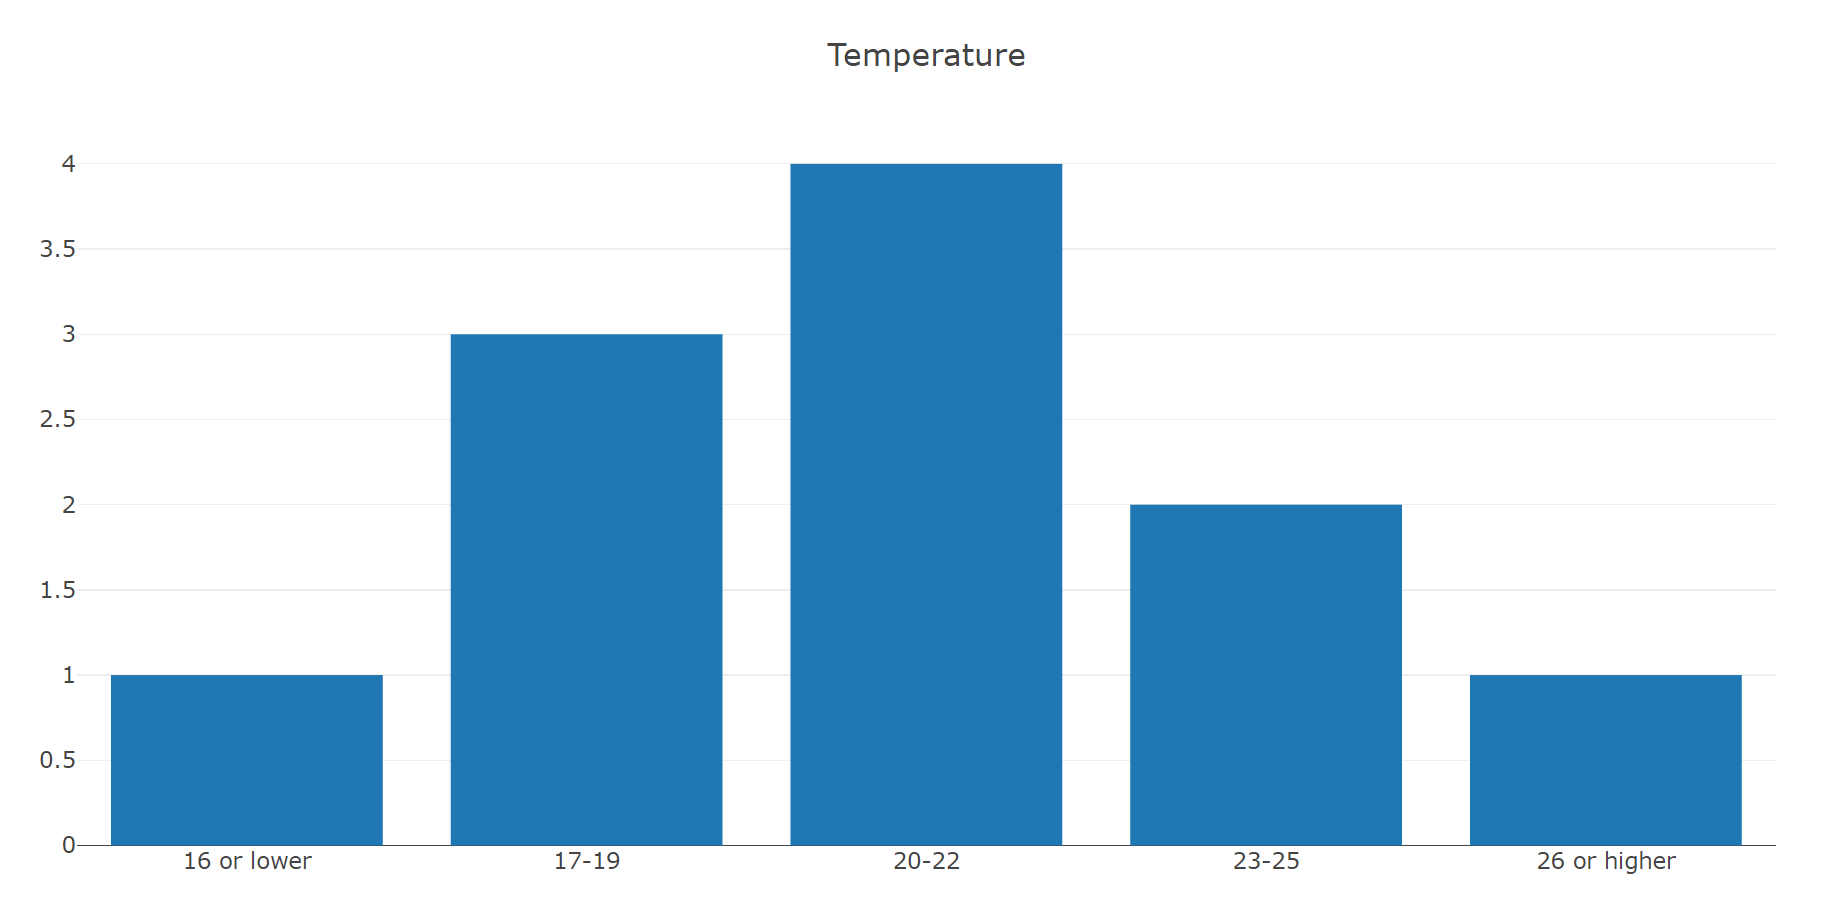
\includegraphics[scale=0.3]{exampleChart.png}
\caption{Histogram temperatury}
\end{figure}

\subsection{Uzyskanie danych za pomocą Telegram botu}

\paragraph{Telegam bot} jest aplikacją wykorzystującą interfejs aplikacji \textit{Telegram}
w celu komunikacji z wybranymi użytkownikami (którzy posiadają możliwość komunikacji ze stworzonym
\textit{bot'em}).\newline
Uzyskane przez platformę dane mogą być wysłane do użytkownika, który ma dostęp do Telegram botu. Dane są wysyłane na żądanie i mogą być jak w postaci tekstu, tak i w postaci obrazu histogramu.



\section{Implementacja}
       
        
        \subsection{Wybór platformy web-serwera}
	Aplikacja internetowa została stworzona za pomocą \textsl{frameworku} \texttt{Flask}. 
	\texttt{Flask} - \textsl{framework} do tworzenia aplikacji internetowych w języku \texttt{Python}, głównie do
	minimalistycznych aplikacji, które celowo zapewniają tylko podstawowe funkcje.
	
    \subsection{Generowanie wykresów w przeglądarce}
	Dla utworzenia wykresów w przeglądarce używana jest biblioteka \texttt{Plotly}, napisana w języku \texttt{JavaScript}.
	Biblioteka pozwala na utworzenie różnorodnych wykresów, z których dla danej aplikacji jest typem \textsl{bar}, odpowiadającym histogramowi. 
	Dane dla wykresów są przekazywane od serwera do przeglądarki jako odpowiedz na żądanie \texttt{HTTP}.

	Żądanie jest obsługiwane w języku \texttt{JavaScript} za pomocą ciągu funkcji, które zostały omówione w dalszej części dokumentacji.

    \subsection{Tworzenie wykresu}
    \begin{lstlisting}[frame=single, numbers=left, basicstyle=\ttfamily\small,
    caption={Funkcja do tworzenia histogramu za pomocą biblioteki \textsl{Plotly.js}}]
function drawChart(chart_divId, chart_title) {
  var trace = {
    type: 'bar',
    x: chartRanges[chart_title],
    y: chartData[chart_title],
  };

  var data = [ trace ];

  chart_title = chart_title.charAt(0).toUpperCase()+chart_title.slice(1);
  var layout = {
    title: chart_title,
    font: {size: 18}
  };

  Plotly.react(chart_divId, data, layout);
}
    \end{lstlisting}

    Dane z serwera są przekazywane w postaci tablicy. 
    Dodatkowym zadaniem skryptu w języku \texttt{JavaScript} jest kategoryzowanie danych
    dla różnych zakresów, zanim wykres będzie stworzony.

    Wartości dla osi \texttt{x} są nazwami zakresów, 
    do których może należeć wartość przekazana z serwera. 
    Dane zakresy są zdefiniowane statyczne i zadeklarowane na samym początku skryptu.
    \begin{lstlisting}[frame=single, numbers=left, basicstyle=\ttfamily\small,
caption={Zdefiniowany zakresy w skrypcie \texttt{JavaScript}}]
chartRanges = {
  "temperature" :
	     ["16 or lower", "17-19", "20-22", "23-25", "26 or higher"],
  "light": 
       ["349 or lower","350-450", "451-550", "551-650", "651 or higher"],
  "humidity":
	  ["0-20", "21-40", "41-60", "61-80", "81-100"]
}
    \end{lstlisting}

\subsection{Asynchroniczne wczytywanie danych z pliku}
    Dane, pobrane z czujników za pomocą platformy \textit{Raspberry Pi}, są przechowywane w pliku z rozszerzeniem \texttt{.csv}.
    Dla asynchronicznego wczytywania danych z pliku została użyty moduł \texttt{watchdog}.
    Dany moduł został użyty do monitorowania wybranych plików. 
    Wybór plików został zdefiniowany za pomocą wyrażeń regularnych. 
    Jeżeli dowolny plik o zadanym rozszerzeniu zostaje zmieniony, to serwer wysyła sygnał do przeglądarki,
    która została połączona z serwerem za pomocą gniazdek i nasłuchuje na te sygnały.
    Do obsługi różnego rodzaju sygnałów jest używany moduł \texttt{flask\_socketio}.
    \begin{lstlisting}[frame=single, numbers=left, basicstyle=\ttfamily\small, language=python,
    caption={Połączenie gniazdka na serwerze z gniazdkiem w przeglądrce}]
@socketio.on('connect')
def test_connect():
global thread
if thread is None:
  thread = socketio.start_background_task(target=background_thread)
    \end{lstlisting}

    Dla każdego sygnału mogą być zdefiniowane osobne funkcje. 
    W danej implementacji sygnał zostaje wysłany 
    jeżeli monitorowany plik został zmieniony. W tym przypadku serwer wysyła sygnał
    do przeglądarki za pomocą funkcji \texttt{on\_modified}, która dodatkowo
    wczytuje dane z pliku, żeby przekazać je do przeglądarki.
   \begin{lstlisting}[frame=single, numbers=left, basicstyle=\ttfamily\small, language=python,
    caption={Definicja wątku, monitorującego zmiany w plikach o zadanym rozszerzeniu}]
def background_thread():
  global observer
  event_handler = CsvWatcher()
  observer = Observer()
  observer.schedule(event_handler, './', recursive=True)
  observer.start()
   \end{lstlisting}

\begin{lstlisting}[frame=single, numbers=left, basicstyle=\ttfamily\small, language=python,
    caption={Definicja funkcji wysyłającej sygnał i dane}]
def on_modified(self,event):
    global csvFileName
    data = readfile(csvFileName)
    socketio.emit('modified', {'data': data})
   \end{lstlisting}

    \subsection{Asynchroniczne odświeżanie wykresów w przeglądarce}
    Asynchroniczne odświeżanie wykresów umożliwia połączenie przeglądarki i serwera za pomocą gniazdek.
    Gniazdka umozliwiają asynchroniczną obsługę sygnałów, wysłanych z serwera.
    
    Do obsługi sygnału w języku \texttt{JavaScript} zostały zdefiniowane następujące funkcję:
\begin{lstlisting}[frame=single, numbers=left, basicstyle=\ttfamily\small,
    caption={Połączenie gniazdek w przeglądrce z serwerem i odebranie danych}]
var socket = io.connect('http://'+document.domain+':'+location.port);

socket.on('modified', function(data) {
    var newData = data['data'];
    start(newData)
});

\end{lstlisting}
\include*{telegram}
\include*{sensors}
\include*{auth}
\include*{raspbian}
\include*{summary}
\end{document}

